% Generated 2020-05-15 16:48:20 -0400
\subsection{Sensor} \label{sec:Sensor}

\gls{sensor term} is a unique type of a piece of equipment.  A \gls{sensor term} is typically comprised of two major components: a \gls{sensor unit} that provides signal processing, conversion, and communications and the \glspl{sensing element} that provides a signal or measured value.

The \gls{sensor unit} is modeled as a \gls{lower level} \gls{component} called \gls{sensor}.  The \gls{sensing element} may be modeled as a \gls{composition} element of a \gls{sensor} element and the measured value would be modeled as a \gls{dataitem} (See \sect{Listing of Data Items} for more information on \gls{dataitem} elements).  Each \gls{sensor unit} may have multiple \glspl{sensing element}; each representing the data for a variety of measured values.

Example:  A pressure transducer could be modeled as a \gls{sensor} (\gls{component}) with a \gls{name} = \textit{Pressure Transducer B} and its measured value could be modeled as a \gls{pressure sample} type \gls{dataitem}.

While a \gls{sensor term} may be modeled in the \gls{xml} document in different ways, it will always be modeled to associate the information measured by each \gls{sensor element} with the \gls{structural element} to which the measured value is most closely associated.   

\subsubsection{Sensor Data}

The most basic implementation of a sensor occurs when the \gls{sensing element} itself is not identified in the data model, but the data that is measured by the \gls{sensing element} is provided as a data item associated with a \gls{component}.  An example would be the measured value of the temperature of a spindle motor.  This would be represented as a \gls{dataitem} called \gls{temperature sample} that is associated with the \gls{rotary} type axis element called "C" as shown in \lst{example-of-sensing-element}:

\newpage 

\begin{lstlisting}[firstnumber=1,escapechar=|,%
    caption={Example of Sensing Element provided as data item associated with a Component}, label={lst:example-of-sensing-element}]
<Components>
    <Axes
        <Components>
            <Rotary id="c" name="C">
                <DataItems>
                    <DataItem type="TEMPERATURE" 
                        id="ctemp" category="SAMPLE" 
                        name="Stemp" units="DEGREE"/>
                </DataItems>
            </Rotary>
        </Components>
    </Axes>
</Components>
\end{lstlisting}

A sensor may measure values associated with any \gls{component} or \gls{device} element.   Some examples of how sensor data may be modeled are represented in \fig{sensor-data-associations}:

\begin{figure}[ht]
  \centering
  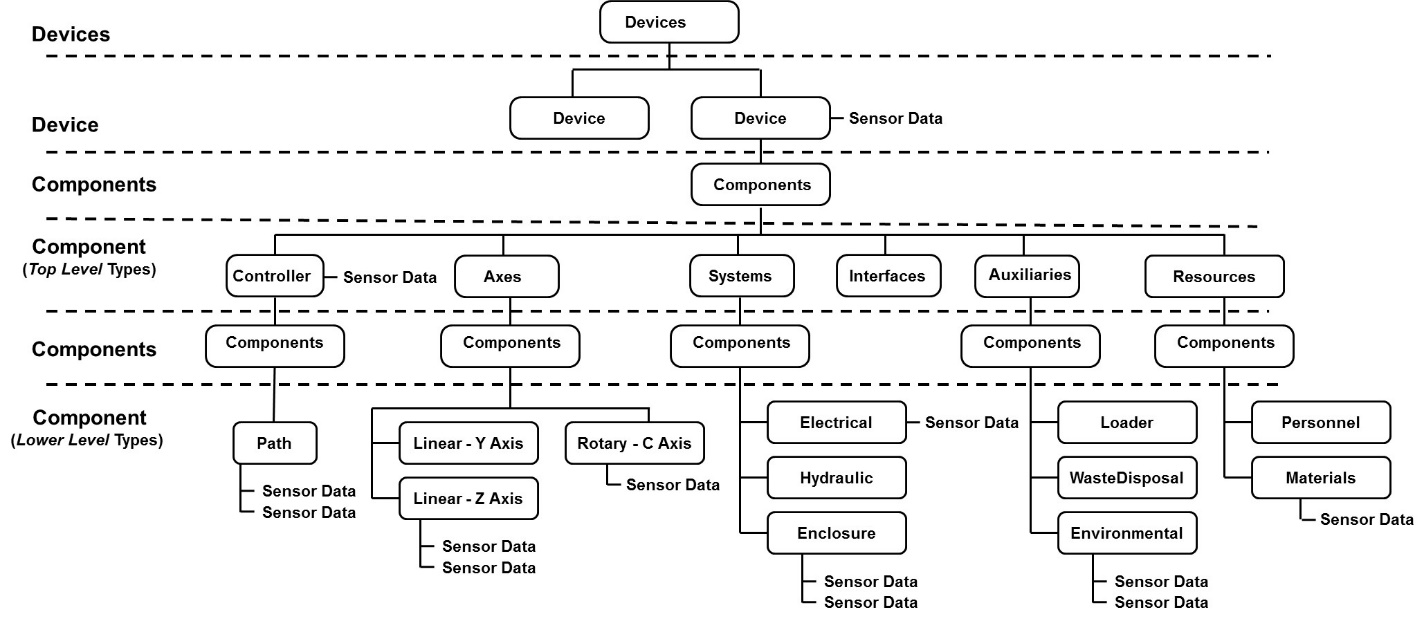
\includegraphics[width=.75\textwidth]{figures/sensor-data-associations.png}
  \caption{Sensor Data Associations}
  \label{fig:sensor-data-associations}
\end{figure}

\subsubsection{Sensor Unit}
\label{sec:Sensor Unit}

A \gls{sensor unit} is an intelligent piece of equipment that manages the functions of one or more \glspl{sensing element}.

Typical functions of the \gls{sensor unit} include:

\begin{itemize}
\item convert low level signals from the \glspl{sensing element} into data that can be used by other pieces of equipment.  (Example:  Convert a non-linear millivolt signal from a temperature sensor into a scaled temperature value that can be transmitted to another piece of equipment.)

\item process \gls{sensing element} data into calculated values.  (Example:  temperature sensor data is converted into calculated values of average temperature, maximum temperature, minimum temperature, etc.)

\item provide calibration and configuration information associated with each \gls{sensing element}

\item monitor the health and integrity of the \glspl{sensing element} and the \gls{sensor unit}.  (Example:  The \gls{sensor unit} may provide diagnostics on each \gls{sensing element} (e.g., open wire detection) and itself (e.g., measure internal temperature of the \gls{sensor unit}).
\end{itemize}

Depending on how the \gls{sensor unit} is used, it may be considered as either an independent piece of equipment and modeled in the \gls{xml} document as a \gls{device}, or it may be modeled as a \gls{top level} \gls{component} called \gls{sensor} if it is integral to a piece of equipment.

A \gls{sensor} \may have its own \gls{uuid} so it can be tracked throughout its lifetime.

The following examples demonstrate how a \gls{sensor term} may be modeled in the \gls{xml} document differently based on how the \gls{sensor term} functions within the overall piece of equipment

Example\#1:   If the \gls{sensor} provides vibration measurement data for the spindle on a piece of equipment, it could be modeled as a \gls{sensor} for rotary axis named C.

\begin{lstlisting}[firstnumber=1,escapechar=|,%
    caption={Example of Sensor for rotary axis}, label={lst:example-of-sensor}]
<Components>
  <Axes
    <Components>
      <Rotary id="c" name="C">
        <Components>
          <Sensor id="spdlm" name="Spindlemonitor">
            <DataItems>
              <DataItem type="DISPLACEMENT" id="cvib"
                category="SAMPLE" name="Svib" 
                units="MILLIMETER"/>
            </DataItems>
          </Sensor >
        <Components>
      </Rotary>
    </Components>
  </Axes>
</Components>
\end{lstlisting}

Example\#2:   If a \gls{sensor} provides measurement data for multiple \gls{component} elements within a piece of equipment and is not associated with any particular \gls{component} element, it \may be modeled in the \gls{xml} document as an independent \gls{lower level} \gls{component} and the data associated with measurements are associated with their associated \gls{component} elements.

This example represents a \gls{sensor unit} with two \glspl{sensing element}, one measures spindle vibration and the other measures the temperature for the X axis.   The \gls{sensor unit} also has a \gls{sensing element} measuring the internal temperature of the \gls{sensor unit}.

\begin{lstlisting}[firstnumber=1,escapechar=|,%
    caption={Example of Sensor Unit with Sensing Element}, label={lst:example-of-sensor-with-sensing-elements}]
<Device id="d1" uuid="HM1" name="HMC_3Axis">
  <Description>3 Axis Mill</Description>
  <Components>
    <Axes
      <Components>
        <Sensor id="sens1" name="Sensorunit">
          <DataItems>
            <DataItem type="TEMPERATURE" id="sentemp"
              category="SAMPLE" name="Sensortemp" 
              units="DEGREE"/> 
          </DataItems>
        </Sensor >
        <Rotary id="c" name="C">
          <DataItems>
            <DataItem type="DISPLACEMENT" id="cvib"
              %category="SAMPLE" name="Svib" 
              units="MILLIMETER">
                <Source componentId="sens1"/>
            <DataItem/>
          </DataItems>
        </Rotary>
        <Linear id="x" name="X">
          <DataItems>
            <DataItem type="TEMPERATURE" id="xt" 
              category="SAMPLE" name="Xtemp" 
              units="DEGREE">
                <Source componentId="sens1"/>
            <DataItem/>
          </DataItems>
        </Linear>
      <Components>
    </Axes>
  </Components>
</Device>
\end{lstlisting}

When a \gls{sensor} unit is modeled in the \gls{xml} document as a \gls{component} or as a separate piece of equipment, it may provide additional configuration information for the \glspl{sensor element} and the \gls{sensor unit} itself.  

\gls{configuration} data provides information required for maintenance and support of the sensor.

\gls{configuration} data is only available when the \gls{sensor} unit is modeled as a \gls{component} or a separate piece of equipment. For details on the modeling of configuration data in the \gls{xml} document, see \sect{Configuration for Component}.

When \gls{sensor} represents the \gls{sensor unit} for multiple \gls{sensing element}(s), each sensing element is represented by a \gls{channel}.   The \gls{sensor unit} itself and each \gls{channel} representing one \gls{sensing element} \may have its own configuration data.

\gls{sensorconfiguration} can contain any descriptive content for a \gls{sensor unit}.  This element is defined to contain mixed content and additional \gls{xml} elements (indicated by the \gls{any} element in \fig{sensorconfiguration-schema-diagram}) \may be added to extend the schema for \gls{sensorconfiguration}.



\subsubsection{Channel}
  \label{sec:Channel}


When \gls{sensor} represents multiple \glspl{sensing element}, each \gls{sensing element} is represented by a \gls{channel} for the \gls{sensor}. 


\paragraph{Attributes of Channel}\mbox{}
\label{sec:Attributes of Channel}

\tbl{attributes of Channel} lists the attributes of \texttt{Channel}.

\begin{table}[ht]
\centering 
  \caption{Attributes of Channel}}
  \label{table:attributes of Channel}
\tabulinesep=3pt
\begin{tabu} to 6in {|l|l|l|} \everyrow{\hline}
\hline
\rowfont\bfseries {Attribute} & {Type} & {Multiplicity} \\
\tabucline[1.5pt]{}
\texttt{name} & \texttt{NMTOKEN} & 0..1 \\
\texttt{number} & \texttt{NMTOKEN} & 1 \\
\end{tabu}
\end{table}
\FloatBarrier


Descriptions for attributes of \texttt{Channel}:

\begin{itemize}
\item \texttt{name} : The name of an element or a piece of equipment.
\item \texttt{number} : A unique identifier that will only refer to a specific {term:sensing element}.
\end{itemize}

\paragraph{Elements of Channel}\mbox{}
\label{sec:Elements of Channel}

\tbl{elements of Channel} lists the elements of \texttt{Channel}.

\begin{table}[ht]
\centering 
  \caption{Elements of Channel}}
  \label{table:elements of Channel}
\tabulinesep=3pt
\begin{tabu} to 6in {|l|l|l|} \everyrow{\hline}
\hline
\rowfont\bfseries {Association Name} & {Element} & {Multiplicity} \\
\tabucline[1.5pt]{}
\texttt{CalibrationDate} & \texttt{dateTime} & 0..1 \\
\texttt{CalibrationInitials} & \texttt{string} & 0..1 \\
\texttt{NextCalibrationDate} & \texttt{dateTime} & 0..1 \\
\texttt{Description} & \texttt{Description} & 0..1 \\
\texttt{Channels} & \texttt{SensorConfiguration} & 1 \\
\end{tabu}
\end{table}
\FloatBarrier


Descriptions for elements of \texttt{Channel}:

\begin{itemize}
\item \texttt{CalibrationDate} : Date upon which the \gls{sensor unit} was last calibrated to the \gls{sensor element}.
\item \texttt{CalibrationInitials} : The initials of the person verifying the validity of the calibration data.
\item \texttt{NextCalibrationDate} : Date upon which the \gls{sensor element} is next scheduled to be calibrated with the \gls{sensor unit}.

\item \texttt{Description} : An element that can contain any descriptive content.
\item \texttt{Channels} : \gls{channels} \glspl{organize} \gls{channel} elements.

\end{itemize}
\FloatBarrier

\subsubsection{SensorConfiguration}
  \label{sec:SensorConfiguration}


\gls{sensorconfiguration} contains configuration information about a \gls{sensor}.


\paragraph{Elements of SensorConfiguration}\mbox{}
\label{sec:Elements of SensorConfiguration}

\tbl{elements of SensorConfiguration} lists the elements of \texttt{SensorConfiguration}.

\begin{table}[ht]
\centering 
  \caption{Elements of SensorConfiguration}}
  \label{table:elements of SensorConfiguration}
\tabulinesep=3pt
\begin{tabu} to 6in {|l|l|l|} \everyrow{\hline}
\hline
\rowfont\bfseries {Association Name} & {Element} & {Multiplicity} \\
\tabucline[1.5pt]{}
\texttt{CalibrationDate} & \texttt{dateTime} & 0..1 \\
\texttt{CalibrationInitials} & \texttt{string} & 0..1 \\
\texttt{FirmwareVersion} & \texttt{string} & 1 \\
\texttt{NextCalibrationDate} & \texttt{dateTime} & 0..1 \\
\texttt{Channels} & \texttt{Channel} & 0..* \\
\end{tabu}
\end{table}
\FloatBarrier


Descriptions for elements of \texttt{SensorConfiguration}:

\begin{itemize}
\item \texttt{CalibrationDate} : Date upon which the \gls{sensor unit} was last calibrated.
\item \texttt{CalibrationInitials} : The initials of the person verifying the validity of the calibration data.
\item \texttt{FirmwareVersion} : Version number for the sensor unit as specified by the manufacturer.

\item \texttt{NextCalibrationDate} : Date upon which the \gls{sensor unit} is next scheduled to be calibrated.
\item \texttt{Channels} : \gls{channels} \glspl{organize} \gls{channel} elements.

\end{itemize}
\FloatBarrier
